\documentclass[12pt,a4paper,titlepage]{article}
\usepackage[latin1]{inputenc}
\usepackage{amsmath}
\usepackage{amsfonts}
\usepackage{amssymb}
\usepackage{braket}
\usepackage{graphicx}
\usepackage{subcaption}
\usepackage{array}
\usepackage{pbox}


\author{Tobias G\"oppel and Sophia Kronthaler}
\title{Theoretical Practical Course in Computational Physics}
\begin{document}

\maketitle

\newpage
\tableofcontents
\newpage


\section{Monte Carlo (MC) integration method} 

The Monte Carlo integration method is quite similar to the Riemann integration method with the subtle difference that one chooses the $x_i$s randomly. This leads to the following approximative formula for the integral:

\begin{equation}
I = \frac{b-a}{N} \sum_{i=0}^{N-1} f(x_i) \xrightarrow{N\rightarrow \infty} \int_a^b\! f(x)\, \mathrm{dx}
\end{equation}
												

We can estimate the integral of the function f by:

\begin{equation}
\int_a^b\! f(x),\mathrm{dx} \approx I \pm Error = V \braket{f} \pm V \sqrt{\frac{\braket{f^2}-\braket{f}^2}{N}} 
\end{equation}

Of course we do not know the standard deviation of f but we can approximate it "on the flight" when performing the Monte Carlo integration. In our program, we assume that the desired accuracy is
reached, when:
\[accuracy \geq \frac{\sqrt{\frac{\braket{f^2}-\braket{f}^2}{N}}}{\braket{f}} \]


As one can see, the error decreases with $\sim \frac{1}{\sqrt{N}}$.
To get an more detailed idea of what determines the error, we should notice that the individual function values at random points $x_i$ one the x-axis are themselvs random numbers.The Integrand, being sum of random numbers is a random number too. The distribution of the integrated values approaches a Gaussian. By using the central limit theorem it can be shown that the following expression holds:

\begin{equation}
\sigma^2(I_N) = \frac{V^2}{N} \int_V \!(f(x) - \braket{f})^2 \mathrm{dx}=\frac{V^2}{N}\sigma^2(f)
\end{equation}

This leads to the important conclusion that the variance of $I_N$ does not depend only on the quantity of random points $N$, but also on the volume $V$ and the variance of the function $\sigma^2(f)$.
To show this characteristic we define the ratio $\rho$.

\[\rho = \frac{N}{V^2}\frac{\sigma^2(I_N)}{\sigma^2(f)}\]

Figure \ref{fig:monte} shows the result by integrating $f(x)=x$ via the Monte Carlo method. Furthermore results for different functions can be found in the appendix \ref{ap:montecarlo}.


\begin{figure}
	\label{fig:monte}
\centering
\caption{$f(x)=x$, volume: $[-1,1]$, ratio: 1.051}
	\begin{minipage}[b]{\linewidth}
		\centering
		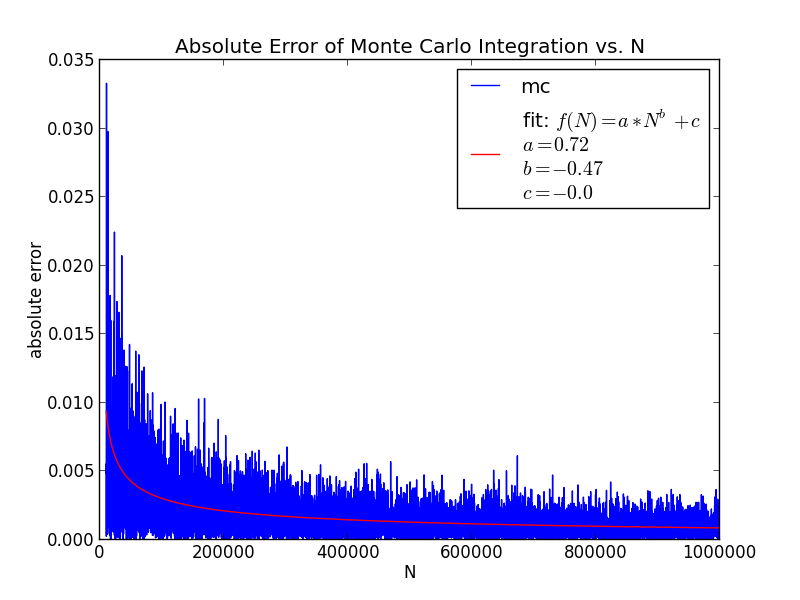
\includegraphics[width=\linewidth]{Plots/linear}
	\end{minipage}
	\begin{minipage}[b]{\linewidth}
		\centering
		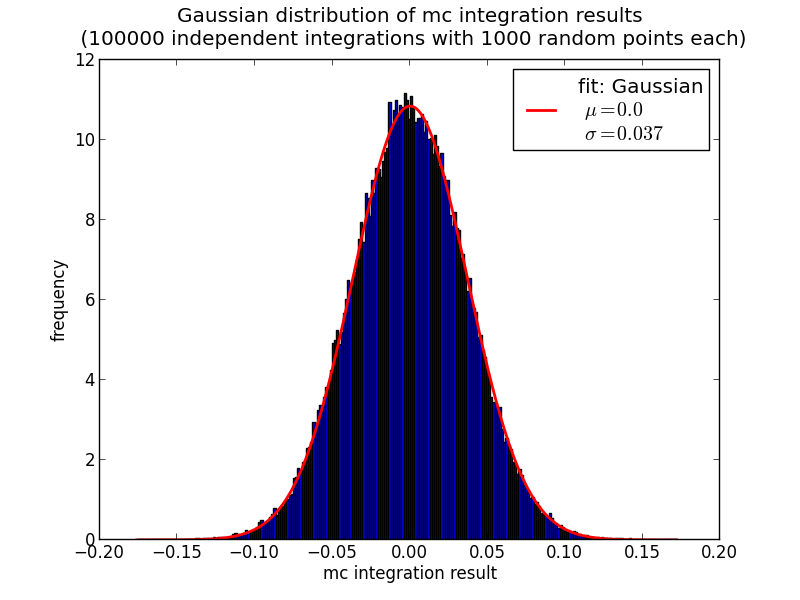
\includegraphics[width=\linewidth]{Plots/linearhist}
	\end{minipage}
\label{fig:linear}
\end{figure}



\newpage
\section{Ising Model}

The Ising model is a well known toy model for ferromagnetism, for that reason it will not be explained in detail here.
The Hamiltonian for a predefined spin configration $\{c\}$ is given by:
 \[H(\{c\})= - \frac{1}{2}\sum_{i=0}^{N-1} \sum_{j=0}^{N-1} J_{ij} s_i s_j - B \sum_{i=0}^{N-1}s_i\]

$J_{ij}$ (coupling term) determines the strength of the force exerted in an interaction of neighboring spins. It depends on the sign of the coupling constant whether the ground state is ordered or disordered. 
\[J_{ij} > 0 \text{the interaction is called ferromagnetic with an ordered GS: } E_0=-NJ\]
\[J_{ij} < 0 \text{the interaction is called anti-ferromagnetic with an disordered GS: } E_0=+NJ\]
In this model we solely consider nearest neighbors interaction with periodic boundary conditions.
With an occupation probability for a specific spin configuration of
\[P(\{c\}) \sim \exp[-\beta H(\vec{S})] \text{with } \beta = \frac{1}{k_B T}\]
one can compute the observables listed below:\newline

\textbf{1d without magnetic field (per spin):}
\begin{align*}
&\braket{u} = \sum_{\{c\}}H(\{c\})P(\{c\}) = -J \tanh(\beta J)\\
&\braket{c} = k_B(\beta J)^2[1-\tanh^2(K)]\\
&\braket{m} = 0 
\end{align*} 


\textbf{1d with magnetic field (per spin):}
\begin{align*}
&\braket{m} = \frac{\sinh(h)}{\sqrt{\sinh^2(h) + \exp(-4\beta J) }}\\
&\braket{\chi}=\beta \cosh(h) \frac{\exp(-4J\beta)}{(\sinh(h)+\exp(-4J\beta))^{\frac{3}{2}}}
\end{align*}


To obtain the exact solution for the 2d Ising Model is a story in itself.\footnote[1]{We recommend the Advanced Statistical Physics Script,
\newline Prof. Dr. Ulrich Schollw\"ock, Chapter 7}







\section{Metropolis Algorithm}

The aim is to generate configurations of Ising systems in thermal equilibrium at a given temperature. The standard method, the Metropolis Algorithm, of acquiring these sample configurations is actually a modified Monte Carlo scheme 'Instead of choosing configurations randomly and then weighting them, we choose configurations with a probability $P\sim \exp(-\frac{E}{k_b T}))$ and weight them evenly.'\cite{metropolis}\newline
The following steps illustrate the Metropolis method:\newline
In the beginning, select some initial spin configuration $\{c^0\}$ and compute its energy $E_0 = H(\{c^0\})$.
Then:


\begin{enumerate}
\item Randomly select one spin $s_i$ of the configuration $\{c\}$
\item Flip $s_i \rightarrow -s_i$ to obtain $\{c^n\} \rightarrow \{c^*\}$
\item Compute the energy $E_*=H(\{c^*\})$ for the new configuration
\item If $E_*\leq E_n$ accept the new configuration $\{c^{n+1}\} = \{c^*\}$
\item Else accept the new configuration with a probability of $\exp(-\beta \bigtriangleup E)$
\item If finally rejected duplicate old configuration $\{c^{n+1}\} = \{c^n\}$
\item Compute $E_{n+1} = H(\{c^{n+1}\})$
\end{enumerate}

To speed up the simulation, we modified these steps by avoiding exponentiations and total energy evaluations inside the metropolis loop.
On that account we calculate the 'acceptance-' or 'weightening-cases' in advance by hand and merely check whichever takes place.
In the beginning, select some initial configuration $\{c^0\}$, compute its energy $E_0 = H(\{c^0\})$, its energy changes by $\bigtriangleup E$ by flipping a spin and its weights $P(\bigtriangleup E)$.
\begin{enumerate}
\item Randomly select one spin $s_i$ of the configuration $\{c\}$
\item Check which case is applicable
\item If it's an 'acceptance-case', flip the spin and calculate the new energy by $E_{n+1} = E_n + \bigtriangleup E$
\item Else accept the new configuration with the applicable probability saved in the weights
\end{enumerate}

The specific cases can be found in Table \ref{tab1d}, \ref{tab1dh}, \ref{tab2d}.


\begin{table}
\centering
\caption{ 1D without magnetic field}

\begin{tabular}{|>{$}c<{$}|>{$}c<{$}|>{$}c<{$}|}
\hline 
\text{case} & \bigtriangleup \text{E} & \text{weight} \\ 
\hline 
+++ \rightarrow +-+ & +8J & exp(-8\beta J) \\ 
\hline 
+-+ \rightarrow +++ & -4J & \text{accept} \\ 
\hline 
+-- \rightarrow ++- & 0 & \text{accept}\\
\hline
\end{tabular}
\label{tab1d}
\end{table}


\begin{table}
\centering
\caption{ 1D with magnetic field (h field is +)}

\begin{tabular}{|>{$}c<{$}|>{$}c<{$}|>{$}l<{$}|}
\hline 
\text{case} & \bigtriangleup \text{E} & \text{weight} \\ 
\hline 
+++ \rightarrow +-+ & 4J +2h & exp(-4\beta J - 2\beta h) \\ 
\hline 
--- \rightarrow -+- & 4J-2h & \text{ if } 4J > 2h \;:\exp(-4\beta J +2\beta h)\; else\; : \text{accept} \\ 
\hline 
+-+ \rightarrow +++ & -4J-2h & \text{accept}\\
\hline
-+- \rightarrow --- & -4J+2h & \text{ if } 4J < 2h \;:\exp(4\beta J -2\beta h)\; else\; : \text{accept}\\
\hline
++- \rightarrow +-- & 2h & \exp(-2\beta h)\\
\hline
--+ \rightarrow -++ & 2h & \text{accept}\\
\hline
\end{tabular} 
\label{tab1dh}
\end{table}


\begin{table}
\centering
\caption{ 2D without magnetic field}

\begin{tabular}{|>{$}c<{$}|>{$}c<{$}|>{$}c<{$}|}
\hline 
\text{case} & \bigtriangleup \text{E} & \text{weight} \\ 
\hline 
\parbox[4em]{1cm}{$+++$\\$+++$\\$+++$} \longrightarrow \pbox{5cm}{$+++$\\$+-+$\\$+++$} & 8J & exp(-8\beta J) \\ 
\hline 
\parbox[4em]{1cm}{$+++$\\$+++$\\$++-$} \longrightarrow \pbox{5cm}{$+++$\\$+-+$\\$++-$} & 4J & exp(-4\beta J) \\ 
\hline 
\parbox[4em]{1cm}{$+++$\\$++-$\\$+-+$} \longrightarrow \pbox{5cm}{$+++$\\$+--$\\$+-+$} & 0 & \text{accept} \\ 
\hline
\parbox[4em]{1cm}{$+++$\\$-+-$\\$+-+$} \longrightarrow \pbox{5cm}{$+++$\\$---$\\$+-+$} & -4J & \text{accept} \\ 
\hline
\parbox[4em]{1cm}{$+-+$\\$-+-$\\$+-+$} \longrightarrow \pbox{5cm}{$+-+$\\$---$\\$+-+$} & -8J & \text{accept} \\ 
\hline

\end{tabular}
\label{tab2d} 
\end{table}
\newpage



\section{Implementation and Performance}

Our implementation of the Ising Model based on the Metropolis Algorithm follows precisely the instructions presented in the previous chapter.
In the beginning an object depending on the initial conditions has to be created, according to the scheme (1D, 1D with external field or 2D) you would like to simulate.
The relationships and heritages, as well as all member functions, are shown in Figure \ref{fig:umlspin}.


\begin{figure}[h]
\centering
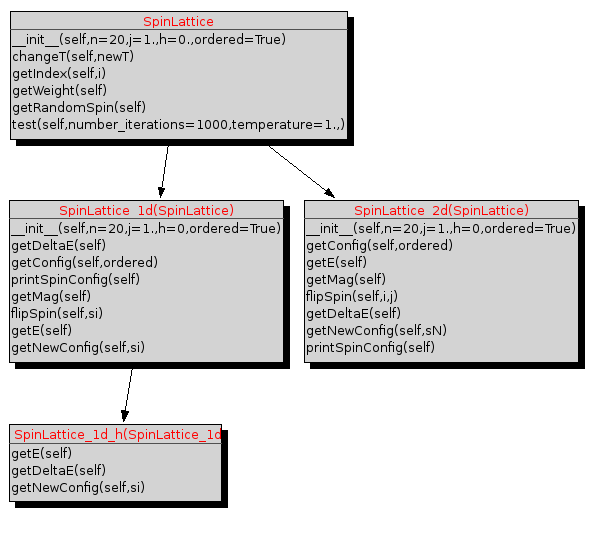
\includegraphics[width=\linewidth]{Plots/umlSpinLattice}
\caption{UML for SpinLattice.py}
\label{fig:umlspin}

\end{figure}

While creating one of these objects, simultaneously the initial spin lattice is formed by calling the $getConfig()$ member function. At that moment the temperature can be defined by the $changeT()$ member function. The next step is to select randomly a spin, check the cases according to the Metropolis rules and finally flip it or not. This functionality is provided by the $getNewConfig()$ method.
We pay particular attention on not evaluating the weights and the total energy inside the metropolis loop. For that reason we compute them once at each temperature step and store them in an array, the $getWeights()$ and $getDeltaE()$ functions are automatically called by the $changeT()$ method.
Since the comparison of tho boolean variables is one of the cheapest operation a computer can perform, we implement the spins as boolean variables (True stands for up and False stands for down).
As the system needs a certain 'time' to reach the thermal equilibrium, we start measuring the observables after several spin flips i.e. several $getNewConfig()$ calls. After the equilibrium is reached we perform several measurements and take the mean afterwards. For convenience we introduce a new parameter named $sweep$, that corresponds to the number of $getNewConfig()$ calls between two successive measurements. For instance for a $100\times100$ lattice we need at least a $sweep \geq 100\times100$. In order to avoid taking non-equilibrium measurements into account and obtaining thereby falsified results, the series of measurements starts after ten sweeps.
To speed up the simulation we used Numpy Arrays, that are known for their faster handling compared to the common Python arrays. Additionally instead of generating another costly random number in the two dimensional case, we recycle the already generated random number by an divmod operation.

\section{Results}


\subsection{One dimension}

From the theory we know that in one dimension the Ising model shows no phase transition for finite temperatures i.e. magnetization is zero for all temperatures except $T=0$. The following Plots (Figures \ref{fig:1denmag},\ref{fig:1dheatsusz}) were generated with a lattice containing $1000$ spins. For temperatures $T\geq 0.5$ our simulation results confirm this behavior Due to finite size effects our simulation wrongly predicts a finite magnetization for small temperatures. To obtain a results closer to the exact solution the spin lattice size should be increased. The $-\tanh(\frac{1}{T})$ dependence of the energy as a function of the temperature could be confirmed quite well. The heat capacity shows as well the theoretically predicted characteristics qualitatively. The susceptibility diverges for $T\rightarrow0$. For a better understanding or visualization Figure \ref{fig:traj1d} shows the dynamics of the lattice configuration during the simulation As one might expect for high temperatures the system remains total disordered, whereas for small temperatures the system clusters.

\begin{figure}

\centering
\begin{tabular}{cc}
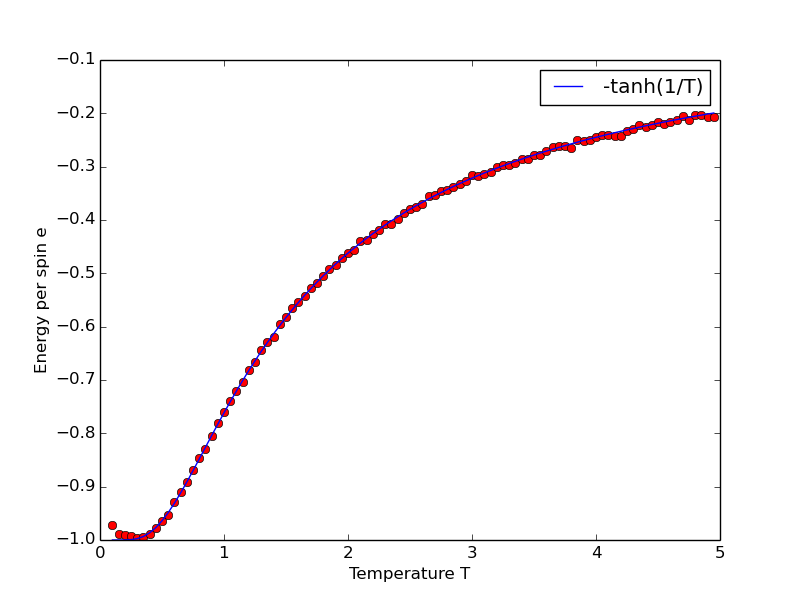
\includegraphics[width=13cm]{Plots/E_Mean_1}\\
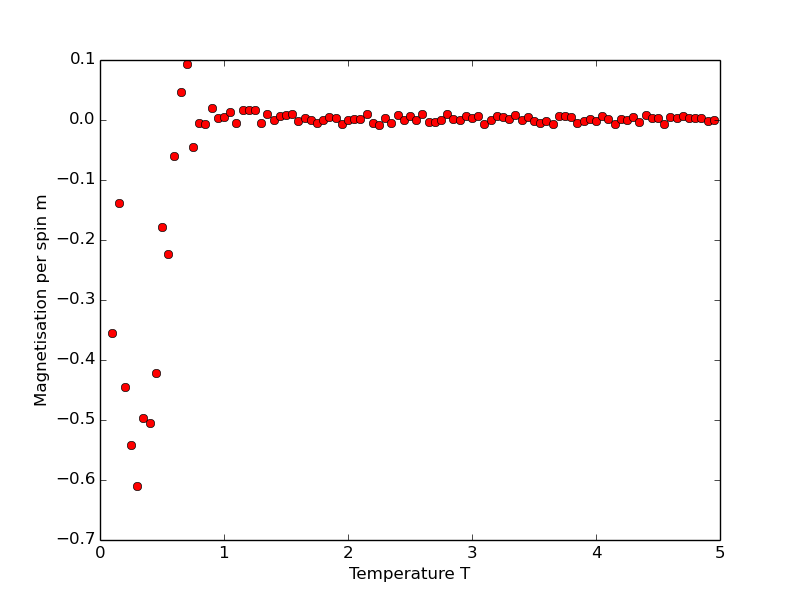
\includegraphics[width=13cm]{Plots/Mag_Mean_1} \\
\end{tabular} 
\caption{Energy and magnetization for 1D without an external field (j=1, sweep: 1000, number of sweeps: 100)}
\label{fig:1denmag}
\end{figure}



\begin{figure}
\centering
\begin{tabular}{cc}
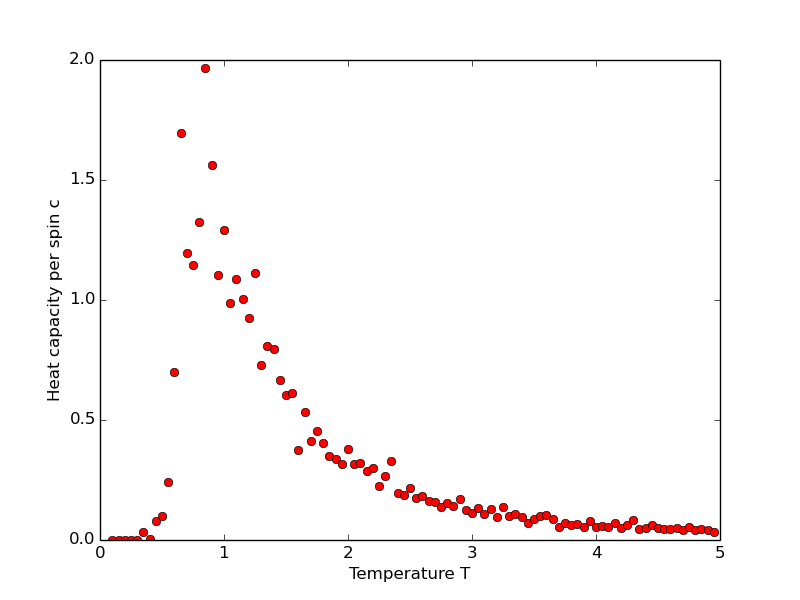
\includegraphics[width=13cm]{Plots/Heat_Capacitiy_1}\\
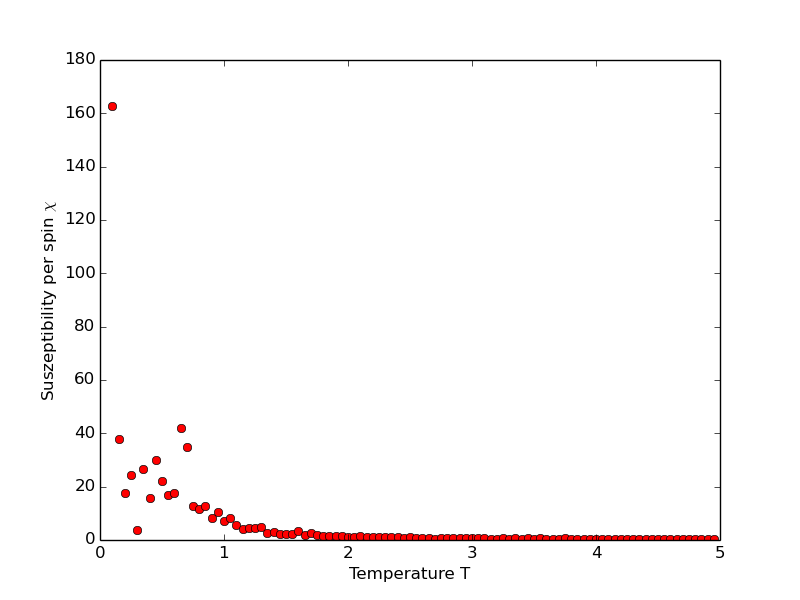
\includegraphics[width=13cm]{Plots/Suszeptibility_1} \\
\end{tabular} 
\caption{Heat capacity and susceptibility for 1D without an external field (j=1, sweep: 1000, number of sweeps: 100)}
\label{fig:1dheatsusz}
\end{figure}

\begin{figure}
\centering

\begin{minipage}[b]{\linewidth}
	\centering
	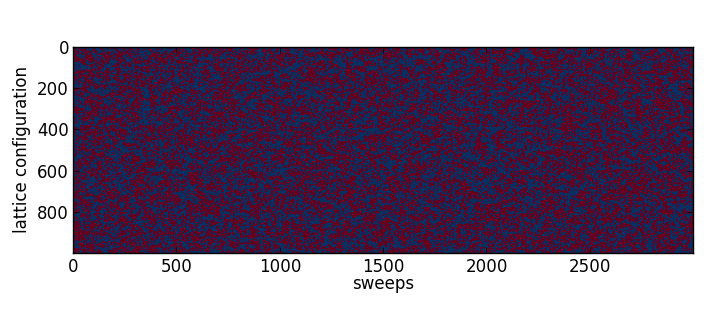
\includegraphics[width=13.6cm]{Plots/Trajectory_1D_1}
\end{minipage}
\begin{minipage}[b]{\linewidth}
	\centering
	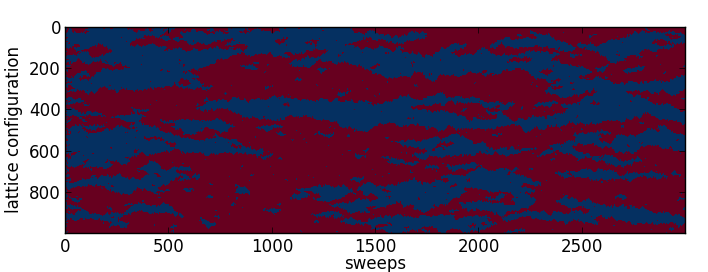
\includegraphics[width=13.5cm]{Plots/Trajectory_1D_05}
\end{minipage}
\begin{minipage}[b]{\linewidth}
	\centering
	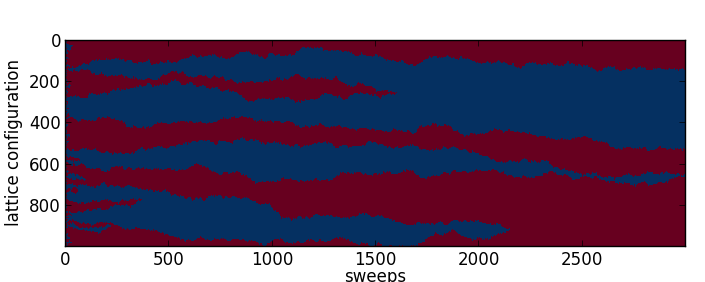
\includegraphics[width=13.45cm]{Plots/Trajectory_1D_02}
\end{minipage}
\caption{Trajectories for the 1D Ising model without an external field for different temperatures: T=1, 0.5, 0.2 and j=1}
\label{fig:traj1d}
\end{figure}

\newpage
\subsection{One dimension with external magnetic field}


The magnetization as a function of the external field should have an sigmoidal shape. From the exact solution we know that for small temperatures the slop for $\braket{m(h=0)}$ increases. For higher temperatures thermal fluctuations work against parallelization of the spins by the external magnetic field. For that reason the system reacts slower on changes of the external field and the linear dependence of the energy on h is not longer valid. Our simulations (Figure \ref{fig:1denmag}, \ref{fig:1denmult}) results confirm these characteristics.



\begin{figure}
\centering
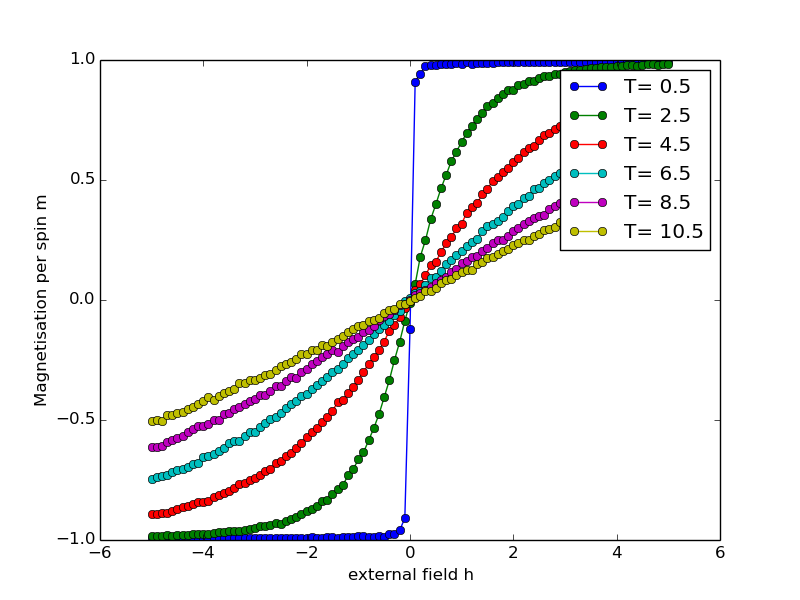
\includegraphics[width=12cm]{Plots/differnt_t_and_h_s_DOTS}
\caption{1D Ising model: magnetization as a function of h for different temperatures}
\label{fig:1dmagmult}
\end{figure}

\begin{figure}
\centering
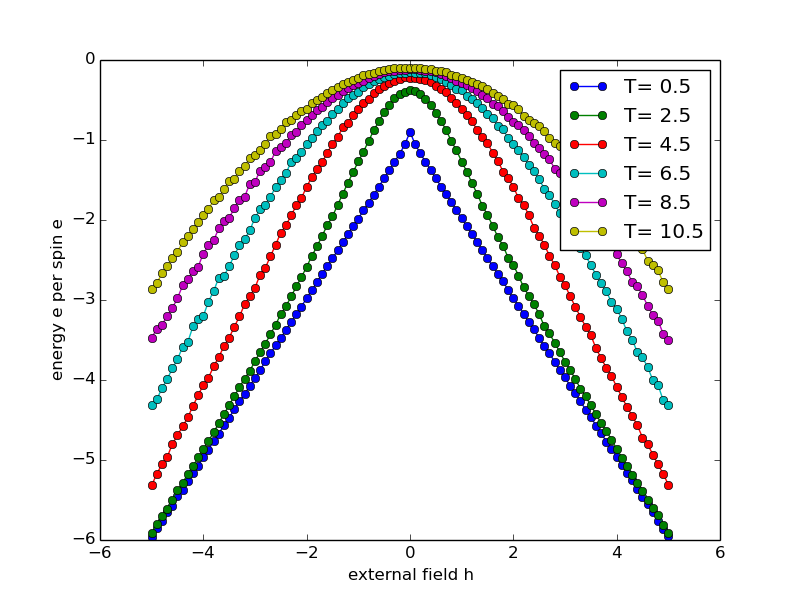
\includegraphics[width=12cm]{Plots/differnt_t_and_h_s_ENERGY}
\caption{1D Ising model: energy as a function of h for different temperatures}
\label{fig:1denmult}
\end{figure}

\begin{figure}
\centering
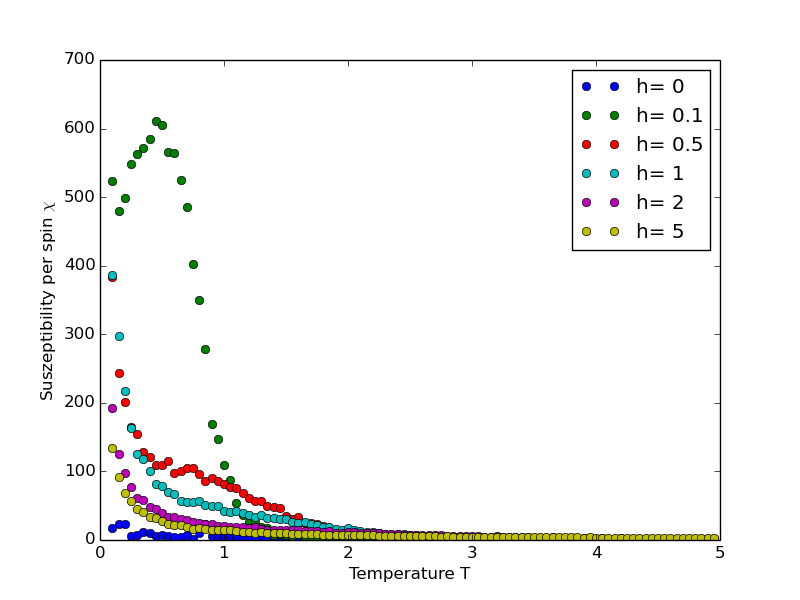
\includegraphics[width=12cm]{Plots/differnt_h_s_10000}
\caption{1D Ising model: susceptibility as a function of h for different temperatures}
\end{figure}




\newpage
\subsection{Two dimensions}


\begin{table}
\centering
\caption{Trajectories for the 2D Ising model without an external field with T= and j=1}
\begin{tabular}{cc}
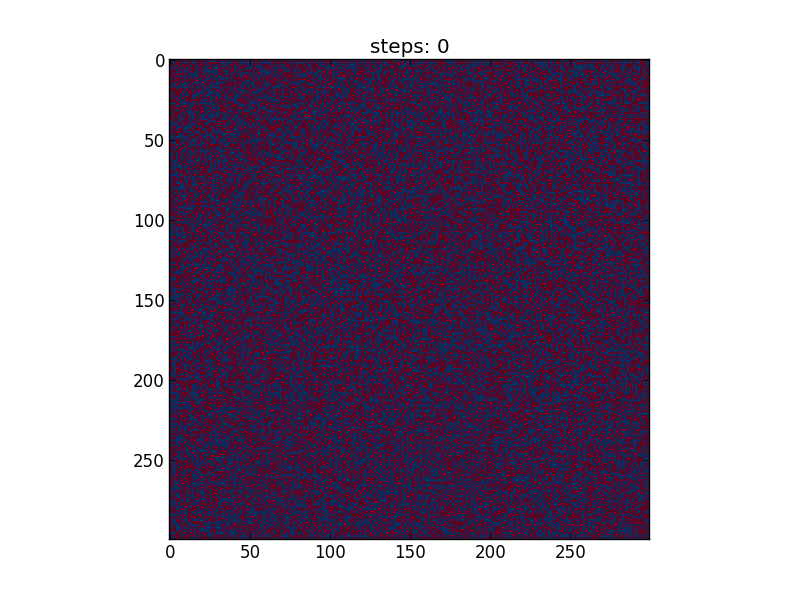
\includegraphics[trim=4cm 0cm 1cm 0cm, width=7cm]{Plots/Trajectory_2D_0} & 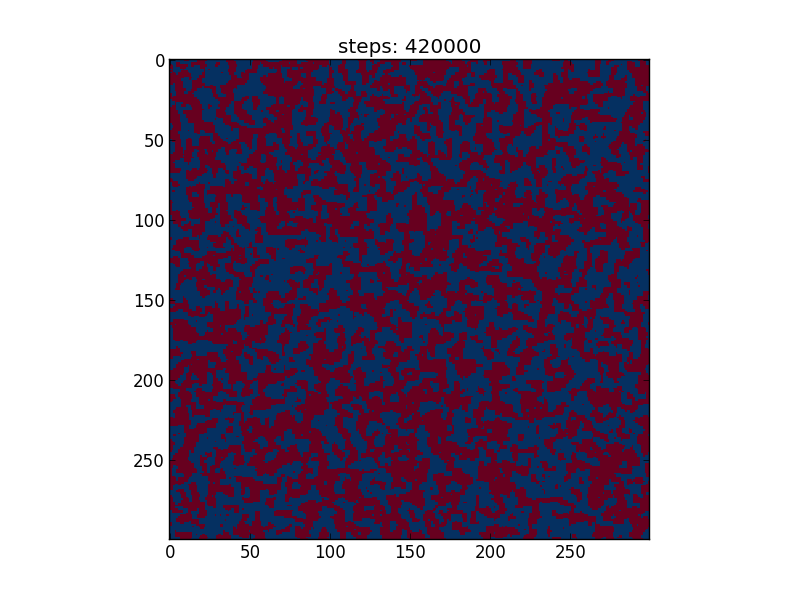
\includegraphics[trim=4cm 0cm 1cm 0cm, width=7cm]{Plots/Trajectory_2D_1} \\
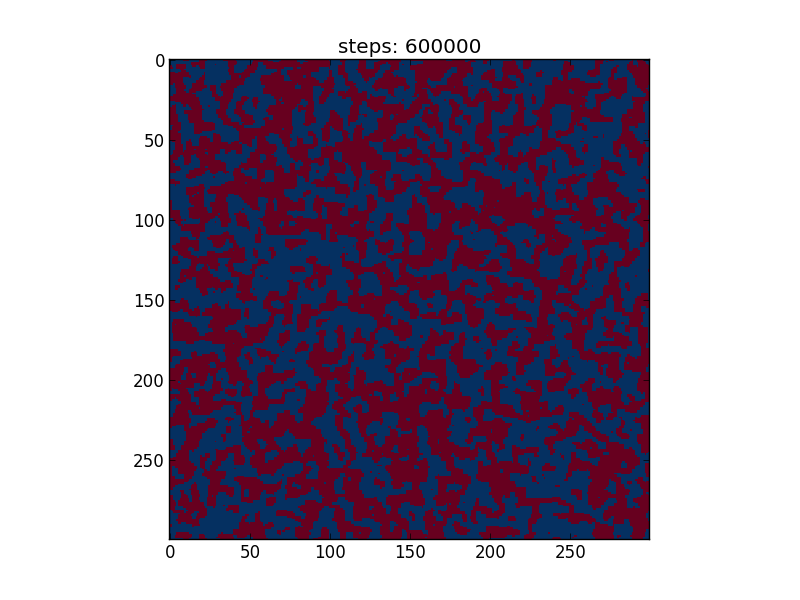
\includegraphics[trim=4cm 0cm 1cm 0cm, width=7cm]{Plots/Trajectory_2D_2} &  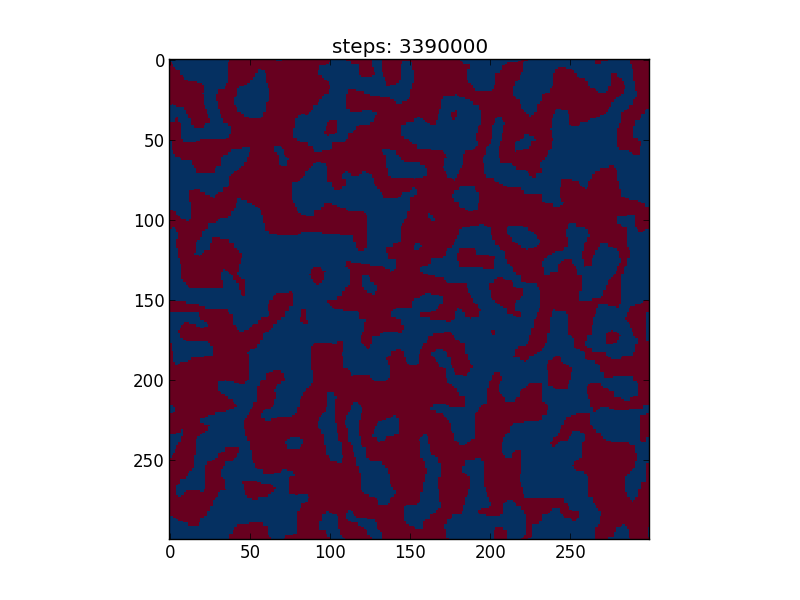
\includegraphics[trim=4cm 0cm 1cm 0cm, width=7cm]{Plots/Trajectory_2D_3} \\
 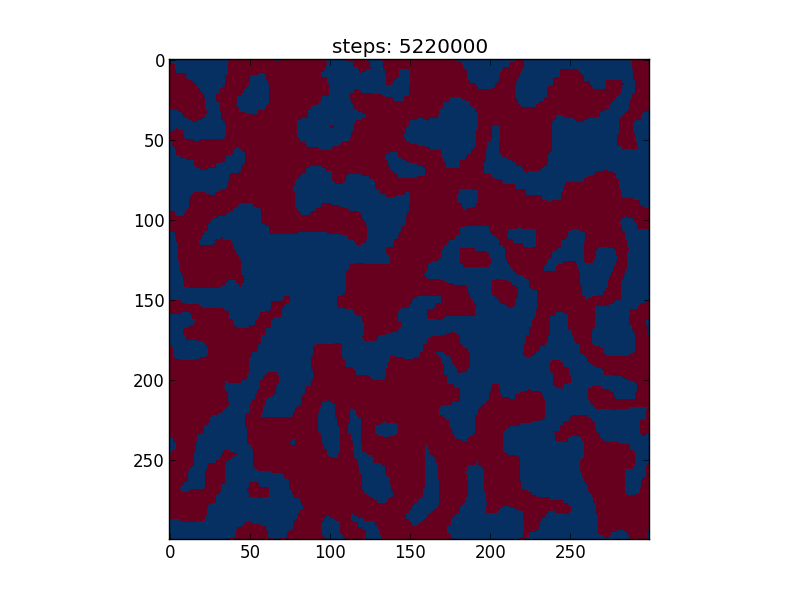
\includegraphics[trim=4cm 0cm 1cm 0cm, width=7cm]{Plots/Trajectory_2D_4} & 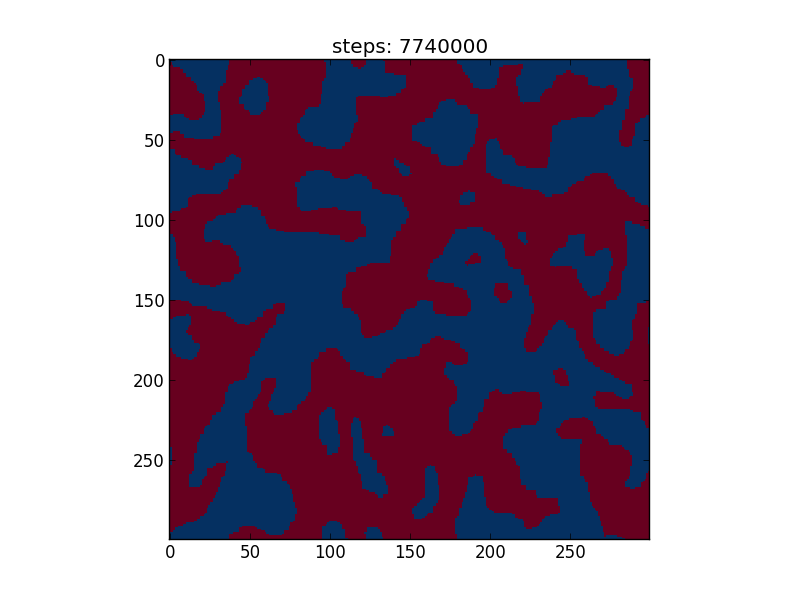
\includegraphics[trim=4cm 0cm 1cm 0cm, width=7cm]{Plots/Trajectory_2D_5} \\
\end{tabular} 

\end{table}



\begin{table}
\centering
\begin{tabular}{cc}
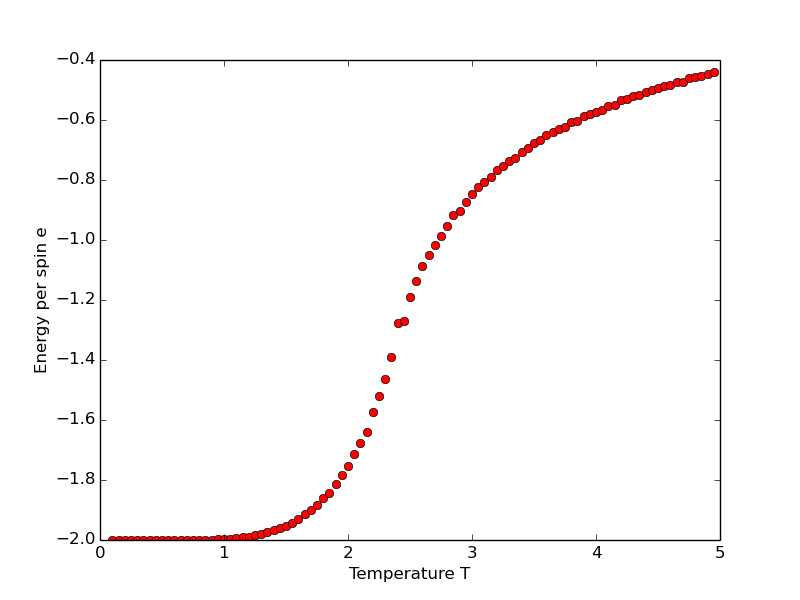
\includegraphics[width=13cm]{Plots/E_Mean_2}\\
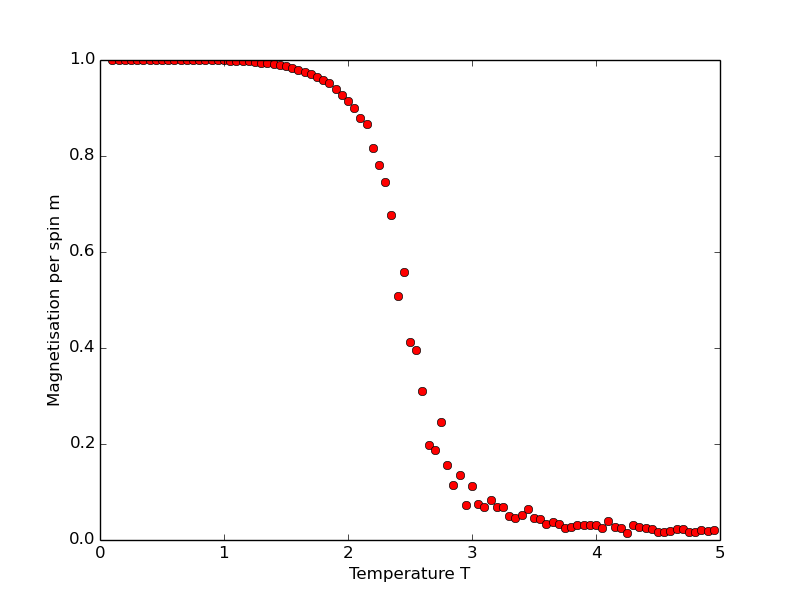
\includegraphics[width=13cm]{Plots/Mag_Mean_2} \\
\end{tabular} 
\caption{Energy and magnetization for 2D without an external field and j=1}
\end{table}



\begin{table}
\centering
\begin{tabular}{cc}
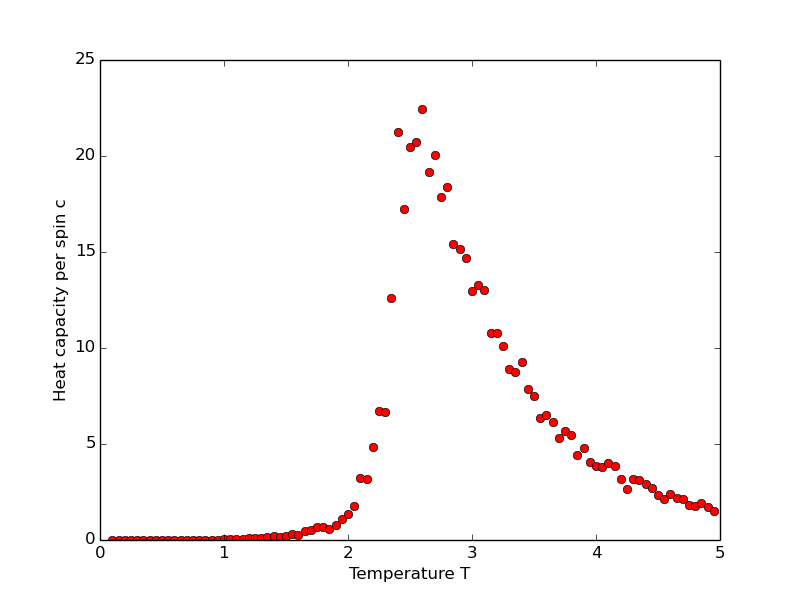
\includegraphics[width=13cm]{Plots/Heat_Capacitiy_2}\\
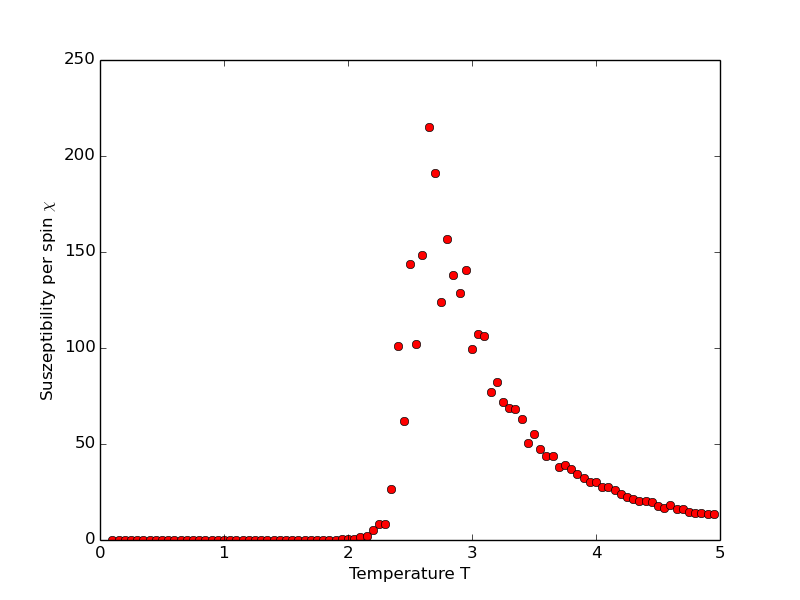
\includegraphics[width=13cm]{Plots/Suszeptibility_2} \\
\end{tabular} 
\caption{Heat capacity and susceptibility for 2D without an external field and j=1}
\end{table}








\begin{thebibliography}{9}


\bibitem{metropolis}

Nicholas Metropolis, Arianna W. Rosenbluth, Marshall N. Rosenbluth, Augusta H. Teller, and Edward
Teller. Equation of state calculations by fast computing machines. The Journal of Chemical Physics, 1953.





\end{thebibliography}

\section{Appendix}
\begin{appendix}
	


\section*{Monte Carlo Plots}

\begin{figure}
	\centering
	\caption{$f(x)=x^2$, volume: $[-1,1]$, ratio: 1.043}
	\begin{minipage}[b]{\linewidth}
		\centering
		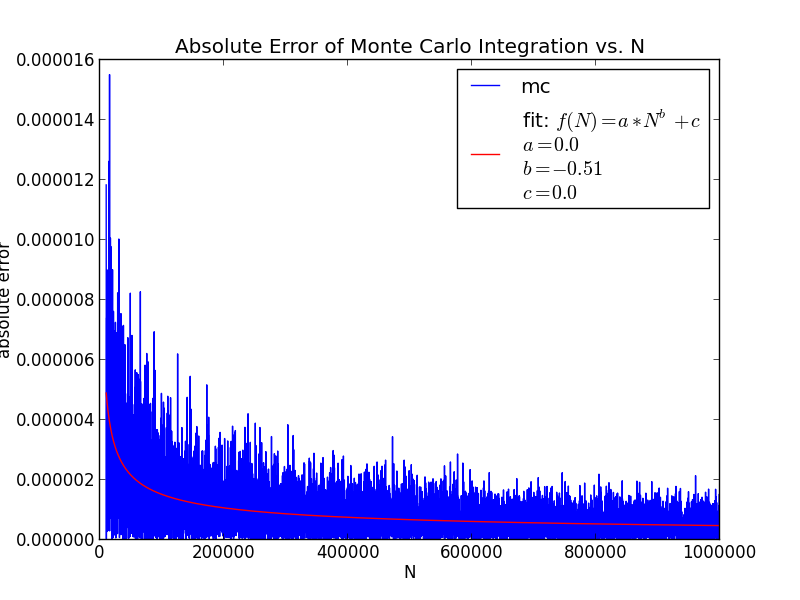
\includegraphics[width=\linewidth]{Plots/quadratisch}
	\end{minipage}
	\begin{minipage}[b]{\linewidth}
		\centering
		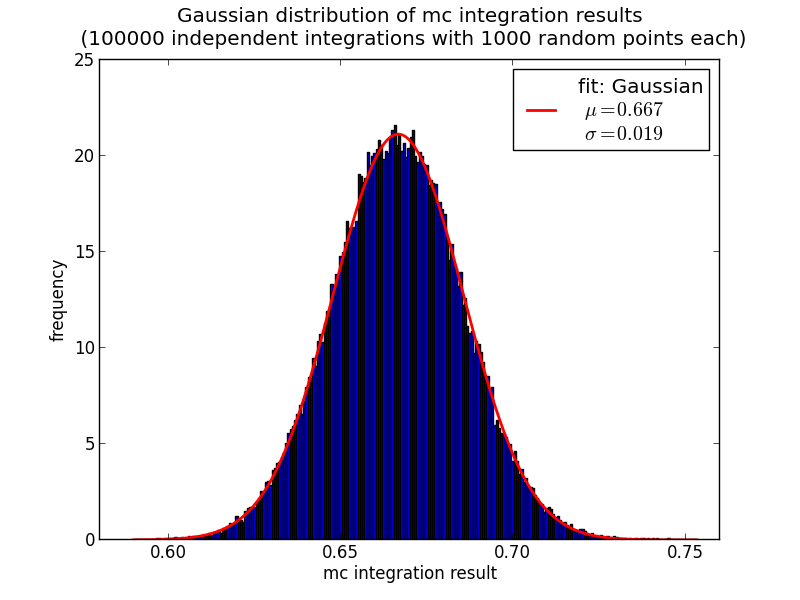
\includegraphics[width=\linewidth]{Plots/histQuadratisch}
	\end{minipage}
	\label{fig:linear}
\end{figure}
\begin{figure}
	\centering
	\caption{$f(x)=x^5$, volume: $[-1,1]$, ratio: 0.951, (the fit function failed to find the correct fit paramters for the Gaussian)}
	\begin{minipage}[b]{\linewidth}
		\centering
		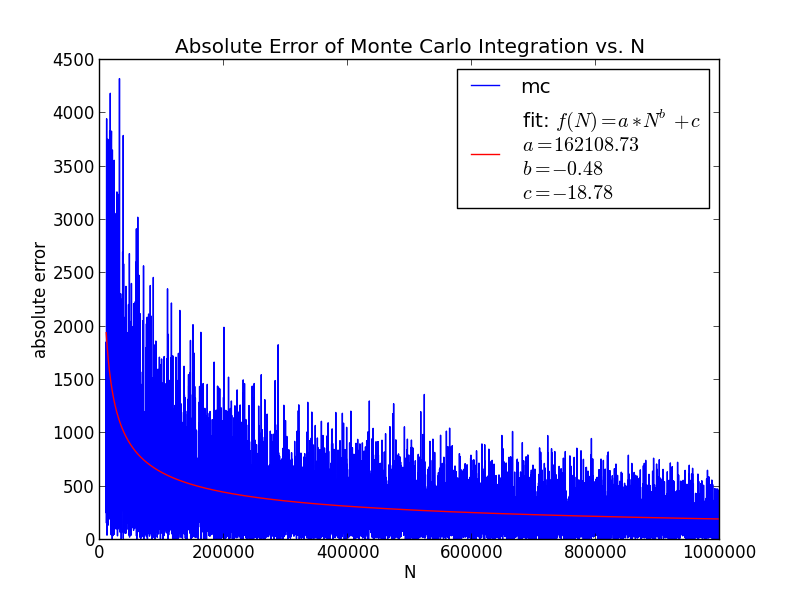
\includegraphics[width=\linewidth]{Plots/x5}
	\end{minipage}
	\begin{minipage}[b]{\linewidth}
		\centering
		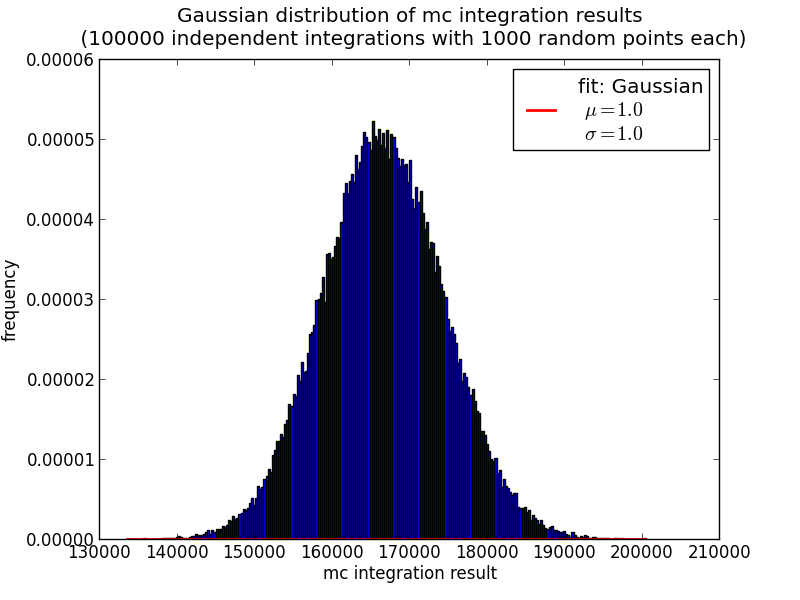
\includegraphics[width=\linewidth]{Plots/x5_HIST}
	\end{minipage}
	\label{fig:linear}
\end{figure}
\begin{figure}
	\centering
	\caption{$f(x)=exp(x)$, volume: $[-1,1]$, ratio: 0.932}
	\begin{minipage}[b]{\linewidth}
		\centering
		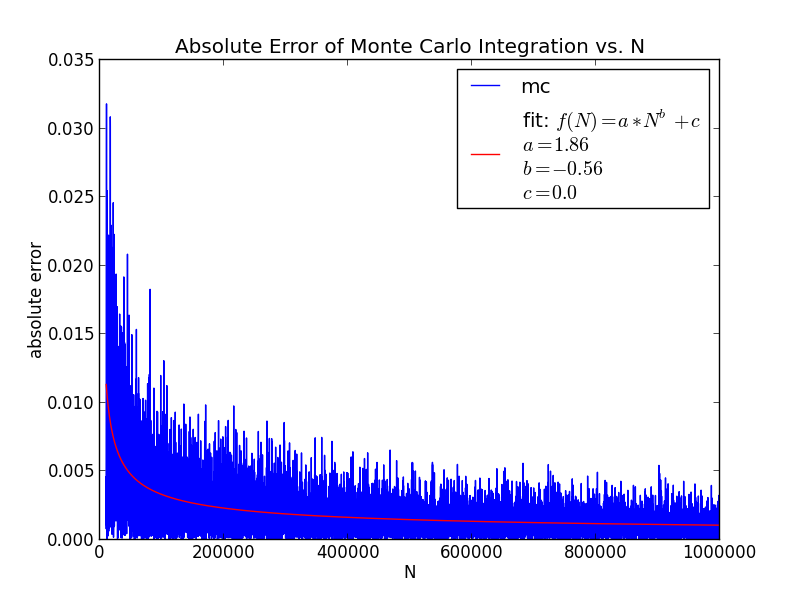
\includegraphics[width=\linewidth]{Plots/eFunktion}
	\end{minipage}
	\begin{minipage}[b]{\linewidth}
		\centering
		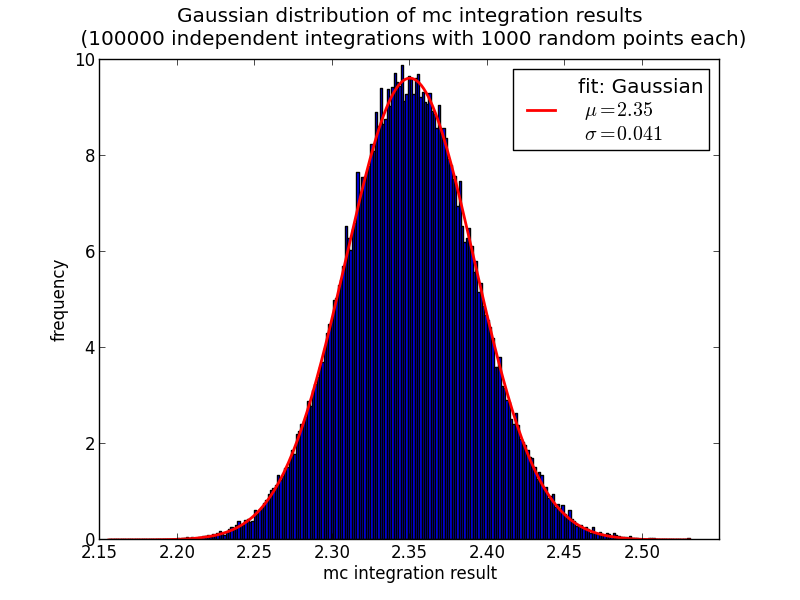
\includegraphics[width=\linewidth]{Plots/eFunktionHist}
	\end{minipage}
	\label{fig:linear}
\end{figure}
\begin{figure}
	\centering
	\caption{$f(x)=sin(x)$, volume: $[0,2\pi]$, ratio: 1.085}
	\begin{minipage}[b]{\linewidth}
		\centering
		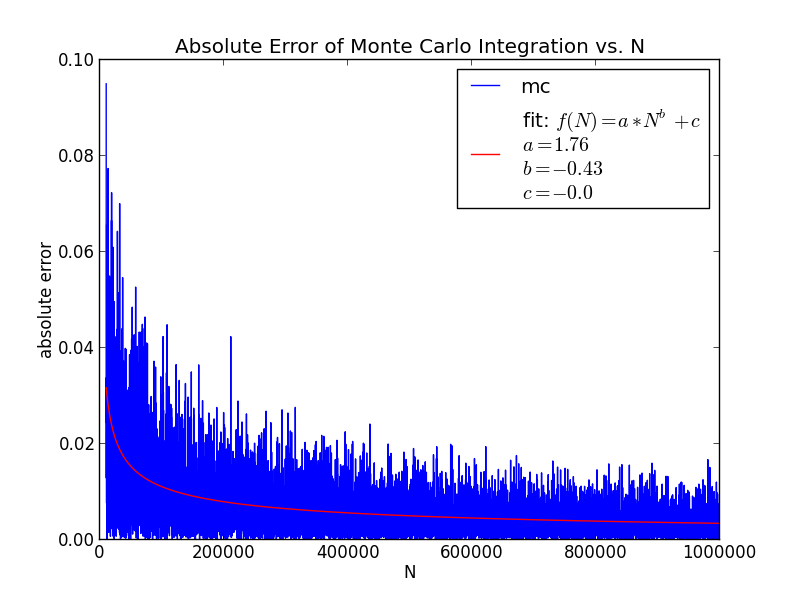
\includegraphics[width=\linewidth]{Plots/sin}
	\end{minipage}
	\begin{minipage}[b]{\linewidth}
		\centering
		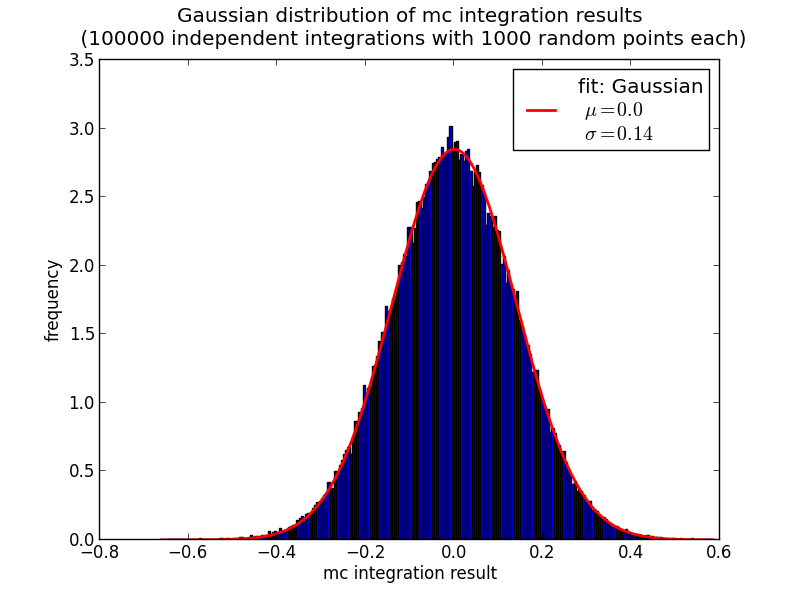
\includegraphics[width=\linewidth]{Plots/sin_hist}
	\end{minipage}
	\label{fig:linear}
\end{figure}


\section*{Code Documentation}
\subsection*{SpinLattice.py}

\end{appendix}


\end{document}
